\documentclass{article}
\usepackage{geometry}
 \geometry{
 a4paper,
 total={170mm,257mm},
 left=20mm,
 top=20mm,
 }
\usepackage{graphicx}
\usepackage{booktabs}
\usepackage{amsmath}
\usepackage{amssymb}
\usepackage{float}
\usepackage{subcaption}
\usepackage[style=authoryear, backend=biber]{biblatex}
\usepackage{xcolor}
\usepackage{hyperref}

\newcommand{\atiyab}[1]{\textcolor{teal}{\textbf{[Atiyab: #1]}}}
\newcommand{\fausto}[1]{\textcolor{blue}{\textbf{[Fausto: #1]}}}
\newcommand{\pia}[1]{\textcolor{purple}{\textbf{[Pia: #1]}}}
\newcommand{\todo}[1]{\textcolor{red}{\textbf{[TODO: #1]}}}

\newenvironment{notes}[1][Note]{\begin{minipage}[t]{\linewidth}\footnotesize{\itshape#1: }}{\end{minipage}}

\addbibresource{refs.bib}

\title{Network Position, Not Network Structure,\\ Shapes Performance in Collective Problem-Solving}
\author{\todo{author list and affiliations}}
\date{August 2026 --- draft for npj Complexity, collection ``Decision-making in Structured Groups''}

\begin{document}
\maketitle

\begin{abstract}
How does the architecture of communication shape collective problem-solving? We study agents on a directed network who face a shared, drifting Boolean-satisfiability task and learn its constraints by \emph{testing} --- verifying candidate rules and re-verifying held beliefs --- and by exchanging signed beliefs (``this constraint exists'' / ``it no longer does''), freshest first. Holding the communication rate equal across networks, we find a sharp dissociation. Network \emph{structure} does not matter: average performance, best-agent performance, and agreement are statistically indistinguishable across random, small-world, scale-free, and layered topologies, and across a thirteen-fold range of network density. Network \emph{position} matters everywhere: an agent's long-run performance falls along a single universal curve in its communication intake, identical across topologies. Structure's real role is to decide \emph{which positions on that curve exist}. Centralised architectures therefore do not raise average performance --- they make individual performance \emph{allocatable}, letting a designer choose who performs best. \todo{add one clause on the analytical result once the derivation is complete}
\end{abstract}


\section{Introduction}\label{sec:intro}

Decision-making under uncertainty is the foremost concern of any organisation. Individuals solve problems with incomplete knowledge, bounded rationality, and asymmetric access to information; what each member knows depends on what the environment supplies and on what neighbours communicate. The architecture that channels this information --- who talks to whom, with what bandwidth, through what intermediaries --- is widely believed to shape not only what a group learns but how fast, by whom, and with what degree of consensus.

Two research traditions make that belief precise, and pull in different directions. A long line in organisation theory treats hierarchical architecture as an efficient response to bounded rationality and costly information processing \parencite{simon1962architecture, radner1993organization, bolton1994firm}: concentrating problem-solving capacity in well-connected nodes reduces the communication an organisation needs. A complementary literature on collective problem-solving in networks finds trade-offs: integrated, centralised networks diffuse good solutions quickly but risk premature convergence, while sparser or more clustered networks preserve the diversity that long-run performance may require \parencite{lazer2007network, mason2008propagation, fang2010balancing, shore2015facts, barkoczi2016social}. A parallel strand on opinion dynamics and social learning asks when structured interaction yields consensus or accuracy \parencite{noorazar2020classical, bala1998learning, jackson2011overview}; \textcite{berekmeri2020optimal} find that consensus favours egalitarian networks while accuracy can favour hierarchical ones in which a few specialists act as information hubs.

Comparisons of this kind face a basic confound: a denser network simply moves more information per unit time, so any performance difference may reflect communication \emph{volume} rather than communication \emph{structure}. We therefore normalise the per-agent communication rate --- the average agent absorbs the same number of messages per period on every network we study --- and ask what architecture still does. The task, following \textcite{hebert2025governance}, is a distributed Boolean-satisfiability problem: all agents choose values for the same $K$ binary variables subject to a hidden set of logical constraints, which they learn piecemeal and which drifts over time, so that knowledge decays and never-resolved problems carry forward. A diagnostic finding motivates the learning model we use. In a predecessor model where agents learn constraints by passive observation and never unlearn, the drifting environment fills knowledge bases with \emph{stale} constraints --- rules that no longer exist but are held, acted on, and endlessly re-transmitted as if new. In long runs, 70--85\% of circulating information is stale, so communication --- the only structure-dependent channel --- carries almost no signal, and no comparison of architectures is informative: whatever the topology, it is a conduit for noise. We therefore equip agents with \emph{verification}: they actively test candidate constraints and re-test what they believe, they retain and transmit disconfirmations (``that requirement was dropped'') alongside discoveries, and they pass on their freshest information first. These mechanisms, natural descriptions of how real problem-solvers probe and gossip, keep the share of stale knowledge low and make communication carry live content --- giving structure its best chance to matter.

It still does not --- but position does. Our results dissociate two questions that the literature usually treats as one. (i) \emph{Structure}: across random, small-world, scale-free, and layered networks matched on communication rate, long-run average performance, best-agent performance, and agreement are statistically indistinguishable; the same holds across a thirteen-fold range of average degree. (ii) \emph{Position}: within every one of those networks, an agent's long-run performance rises steadily with its in-degree, and the relationship collapses onto a \emph{single universal curve} --- performance as a function of communication intake --- shared by all topologies. Structure's role is thereby reduced to something precise: it determines \emph{which positions on the universal curve exist}. A degree-homogeneous network offers only positions near the average; a centralised one manufactures high-intake seats far up the curve, occupied by whomever the designer chooses. Centralisation, on this account, buys not average performance but \emph{intentionality} --- the ability to decide where in the organisation excellence sits, which is valuable precisely when decision rights, attention, or control are scarce. \todo{one sentence previewing the analytical derivation once complete}

\section{Results}\label{sec:results}

\subsection{The model}\label{sec:model}

$N$ agents sit on a fixed directed graph. All face the same task: each agent $i$ privately chooses an assignment $x^{(i)} \in \{0,1\}^K$ of $K$ binary variables, which the environment scores against a hidden set $\mathcal{C}$ of $M = \alpha K$ logical clauses, each an \textsc{and} or \textsc{xor} over two variables (50/50 mix), drawn from the universe $\mathcal{U}$ of the $K(K-1)$ possible such clauses. An agent's performance is its \emph{violation count}: the number of clauses of $\mathcal{C}$ its assignment violates (lower is better). The environment drifts: every $\tau$ ticks one clause of $\mathcal{C}$ is replaced.

Agents hold \emph{signed beliefs} about clauses: a positive belief (``this constraint exists'') or a negative one (``it does not''), stored with capacity $2M$. Each tick an agent does two things.

\emph{Testing.} With equal probability it either tests a \emph{new} candidate clause drawn at random from $\mathcal{U}$ --- adopting it as a positive belief if the clause really is in $\mathcal{C}$ --- or re-tests a belief it already holds, setting it to the ground truth: a positive belief whose clause has been retired flips to negative (the constraint is \emph{falsified}, but remembered as such), a negative belief whose clause has returned flips back. Whenever a clause becomes an active constraint for the agent, it runs a local greedy repair: it flips each variable of that clause if and only if the flip strictly reduces violations against its positive beliefs.

\emph{Communication.} For each in-neighbour, with a probability normalised so that the \emph{population-average} intake is one message per tick regardless of topology (Methods), the agent pulls the neighbour's \emph{most recently acquired} belief among those on which the two disagree, and adopts the neighbour's sign. Both polarities travel: fresh discoveries and fresh disconfirmations propagate by the same channel, freshest first.

Only positive beliefs constrain action; negative beliefs are epistemic --- they block re-adoption of dead rules and carry disconfirmation to others. The full specification, parameter values, and design rationale are given in Methods. Unless stated otherwise, $N=80$--$101$, $K=30$, $\alpha=2$, fast drift $\tau=1$, horizon $T=2000$ with long-run statistics averaged over the final $500$ ticks, and $\geq 8$ random seeds per condition.

\subsection{Verification keeps collective knowledge live}\label{sec:stale}

Figure~\ref{fig:stale} shows why verification is the precondition for any meaningful comparison of architectures. In the predecessor model (passive observation, no unlearning), the share of held knowledge that is stale grows without bound, reaching ${\sim}74\%$ by $t=2000$ at slow drift ($\tau=10$) and 80--85\% at fast drift ($\tau=1$): communication becomes a rumour mill for dead rules. Testing alone cuts the long-run stale share to ${\sim}20\%$ --- falsified constraints are remembered and their disconfirmation spreads --- and transmitting freshest-first roughly halves the remainder (${\sim}10\%$): stale information now disappears within a few hundred ticks of a clause's death instead of persisting indefinitely.

\begin{figure}[H]
  \centering
  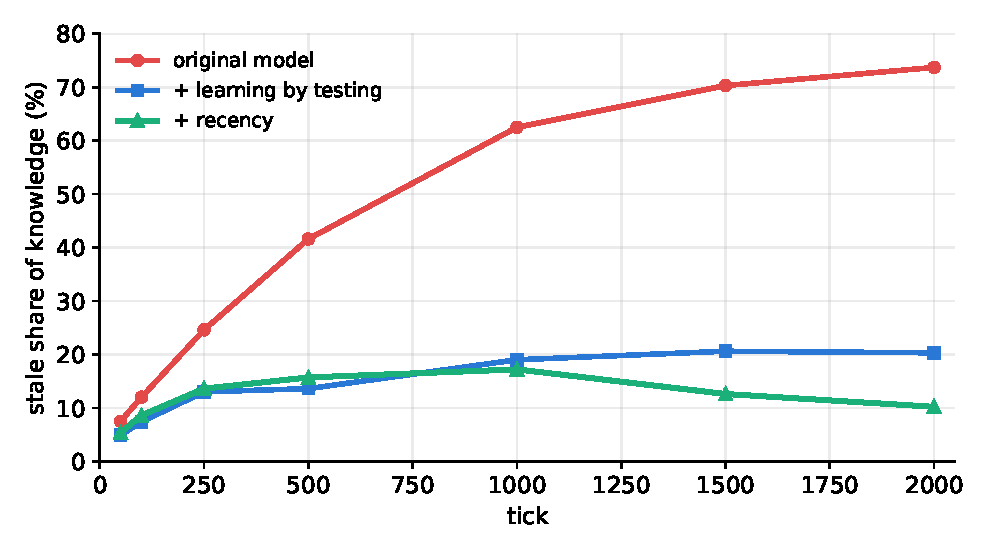
\includegraphics[width=0.62\linewidth]{figs/stale_trajectory.pdf}
  \caption{\textbf{Verification flushes stale information.} Share of held (positive) beliefs whose clause no longer exists, over time. Original model: passive observation, no unlearning. Adding learning by testing retains falsified clauses as transmissible negative beliefs; adding communication recency forwards freshest beliefs first. Scale-free network, $\tau=10$, means over five seeds; each tweak is added on top of the previous.}
  \label{fig:stale}
\end{figure}

\subsection{Network structure does not shape long-run performance}\label{sec:h1}

We first compare four canonical topologies --- scale-free (Barab\'asi--Albert, \cite{barabasi2003scale}), random (Erd\H{o}s--R\'enyi, \cite{erdds1959random}), small-world (Watts--Strogatz, \cite{watts1998collective}), and a layered ``hierarchical'' generator --- matched on average in-degree ($\langle k_{\text{in}}\rangle \approx 4$) and on communication rate, over ten seeds. Long-run performance is statistically indistinguishable across them (Table~\ref{tab:h1}, Fig.~\ref{fig:h1}): average violations span $28.9$--$29.6$ (between-topology spread well within seed noise), best-agent violations $20.2$--$20.4$, and homogeneity --- the average share of agents agreeing on a variable's value --- $0.69$--$0.72$. The one systematic wrinkle is that scale-free networks are \emph{marginally worst} on average ($+0.5$), a point we return to below: their excellent hubs are paid for by a large, poorly connected periphery.

\begin{table}[H]
\centering
\caption{Long-run population metrics by topology (default model; $\tau=1$; time-averaged over the final 500 of 2000 ticks; mean $\pm$ 1 s.d.\ over 10 seeds; homogeneity over 5 seeds). Topologies matched on $\langle k_{\text{in}}\rangle \approx 4$ and normalised communication rate.}
\label{tab:h1}
\small
\begin{tabular}{@{}lccc@{}}
\toprule
Network & Average violations & Best-agent violations & Homogeneity \\
\midrule
Scale-free   & $29.6 \pm 0.4$ & $20.2 \pm 0.6$ & $0.693 \pm 0.010$ \\
Random       & $29.1 \pm 0.7$ & $20.4 \pm 0.8$ & $0.717 \pm 0.017$ \\
Small-world  & $28.9 \pm 0.5$ & $20.3 \pm 0.6$ & $0.710 \pm 0.027$ \\
Hierarchical & $29.3 \pm 0.6$ & $20.3 \pm 0.7$ & $0.706 \pm 0.015$ \\
\bottomrule
\end{tabular}
\end{table}

\begin{figure}[H]
  \centering
  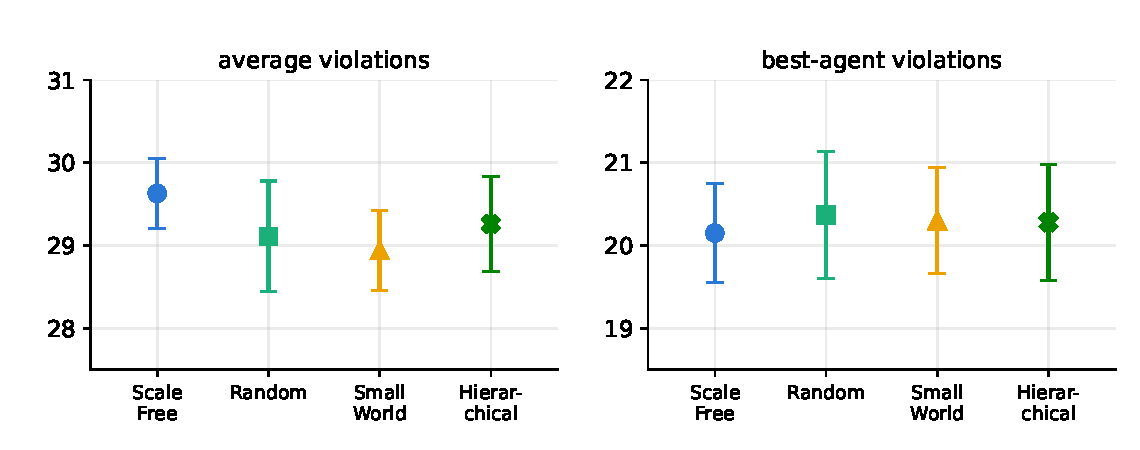
\includegraphics[width=0.85\linewidth]{figs/h1_topology.pdf}
  \caption{\textbf{Structure does not move the population.} Average (left) and best-agent (right) long-run violations by topology; points are seed means $\pm$ 1 s.d. All four topologies are matched on average in-degree and communication rate.}
  \label{fig:h1}
\end{figure}

This is not an artefact of the learning mechanism: the same null result holds in the predecessor model (Methods), where we first observed it and initially suspected stale information as its cause. Verification removes the staleness and the null survives --- topology-independence of the long-run average is a robust property of this class of models once communication volume is controlled.

\subsection{Network position sets individual performance along a universal curve}\label{sec:h2}

Within every network, however, position matters strongly. The rate normalisation fixes the \emph{population-average} intake at one message per tick, not each agent's: an individual's intake remains proportional to its own in-degree. Under drift, more intake means fresher knowledge, and fresher knowledge means fewer violations. Across all four topologies and all ten seeds, agents' long-run violations correlate negatively with in-degree (Spearman $\rho \approx -0.5$ to $-0.6$; negative in 40 of 40 runs), and the eight most central agents outperform the eight least central by $3$--$5$ violations (Table~\ref{tab:h2}). The best-performing agent sits at the 95th centrality percentile in scale-free networks --- in a centralised structure, \emph{who will perform best is predictable from the wiring diagram}.

\begin{table}[H]
\centering
\caption{Position predicts individual performance in every topology (default model; 10 seeds; mean $\pm$ 1 s.d.). $\rho$: Spearman correlation between in-degree and long-run violations. Gap: mean violations of the 8 most central minus the 8 least central agents (negative = central agents better). Best-agent percentile: centrality percentile of the best performer.}
\label{tab:h2}
\small
\begin{tabular}{@{}lccc@{}}
\toprule
Network & $\rho(k_{\text{in}}, V)$ & Gap (top 8 $-$ bottom 8) & Best-agent percentile \\
\midrule
Scale-free   & $-0.61 \pm 0.09$ & $-4.8 \pm 1.1$ & 95\% \\
Random       & $-0.57 \pm 0.09$ & $-3.6 \pm 0.7$ & 88\% \\
Small-world  & $-0.49 \pm 0.10$ & $-3.2 \pm 0.7$ & 71\% \\
Hierarchical & $-0.62 \pm 0.08$ & $-4.3 \pm 0.9$ & 88\% \\
\bottomrule
\end{tabular}
\end{table}

The striking regularity is that the position--performance relationship is the \emph{same} everywhere. Figure~\ref{fig:curve} pools 3{,}200 agent histories: at any given in-degree, mean violations agree across topologies to within a few tenths --- one curve, from ${\sim}31$ violations at the periphery ($k \leq 1$) through ${\sim}27.7$ at $k=8$ down to ${\sim}25$ on the hub tail ($k \geq 19$) that only the scale-free network possesses (shaded). Structure does not bend the curve; it decides which points on it are populated.

\begin{figure}[H]
  \centering
  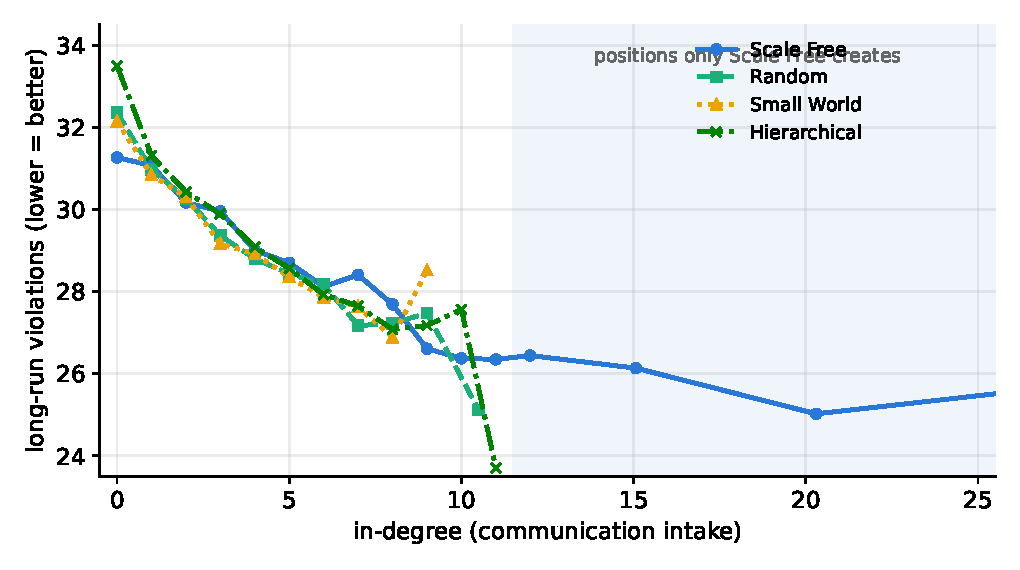
\includegraphics[width=0.72\linewidth]{figs/curve_lbt.pdf}
  \caption{\textbf{One universal position--performance curve.} Per-agent long-run violations versus in-degree, pooled over 10 seeds per topology (bins with $n \geq 5$ agents). All four matched-degree topologies trace the same declining curve; the shaded region marks in-degrees that only the scale-free topology creates.}
  \label{fig:curve}
\end{figure}

Figure~\ref{fig:multinet} makes both findings visible at once, and extends them far beyond matched density. We add two designed networks with uniform in-degree distributions (spanning $1$--$10$ and $1$--$100$) to the natural topologies, so that average degree now ranges from ${\sim}4$ to ${\sim}50$. Within each network, violations decline with in-degree --- with a slope inversely proportional to the network's average degree, exactly as rate normalisation predicts (a given in-degree buys intake $k/\langle k_{\text{in}}\rangle$; plotted against intake, all curves collapse onto one, Fig.~\ref{fig:collapse}). Across networks, the population averages (crosses) are flat: a least-squares fit through them has slope $-0.002$ violations per unit of average degree ($r=-0.11$) across the thirteen-fold density range. Every network's average agent sits at the same point of the same curve; networks differ only in how far their extremes reach along it.

\begin{figure}[H]
  \centering
  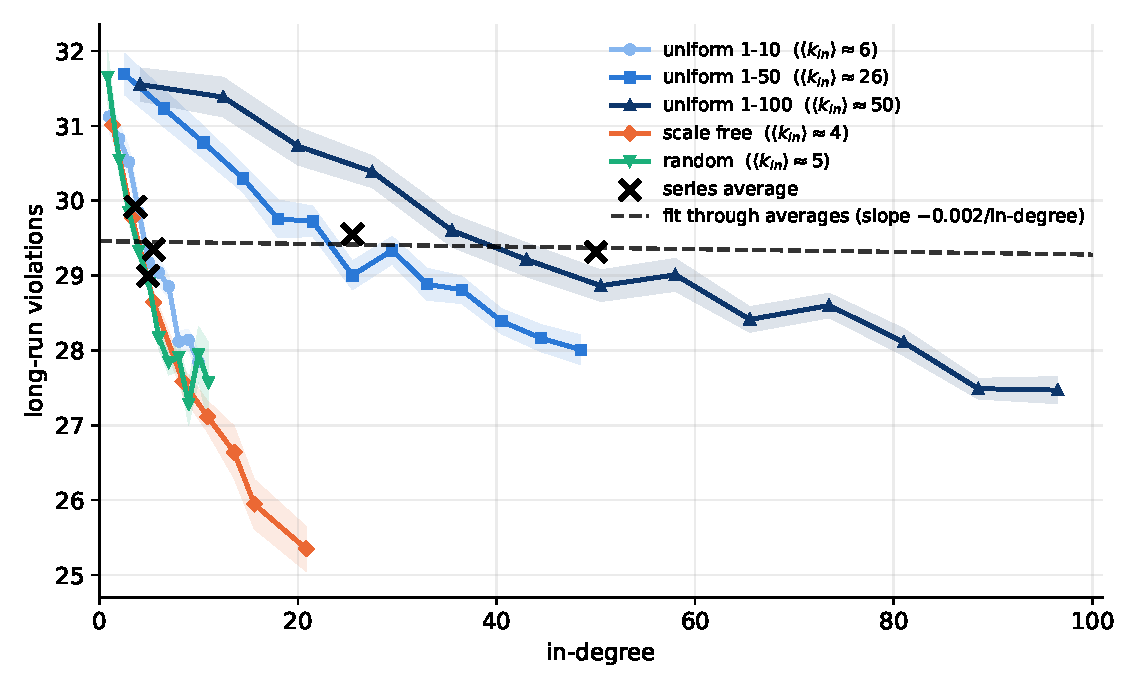
\includegraphics[width=0.8\linewidth]{figs/curve_multinet_degree.pdf}
  \caption{\textbf{Position matters within every network; structure does not matter across them.} Long-run violations versus in-degree for five networks spanning a thirteen-fold range of average degree (natural and designed uniform-degree topologies; default model; $\geq 8$ seeds each; shaded bands $\pm 1$ s.e.m.). Crosses mark each network's population average; the dashed line is the least-squares fit through the crosses (slope $-0.002$, $r=-0.11$).}
  \label{fig:multinet}
\end{figure}

\subsection{Verification is what makes position pay}\label{sec:whytesting}

The position gradient is conditional on trustworthy communication. Repeating the analysis with verification switched off (passive observation, no unlearning --- but the same freshest-first communication) collapses the universal curve into a cliff and a plateau (Fig.~\ref{fig:compare}): being connected at all matters ($34.7$ violations at $k=0$ versus $31.6$ at $k=1$), but beyond the first link additional intake buys almost nothing ($30.2$ at $k=8$; $28.8$ at $k=20$), because ${\sim}80\%$ of what arrives is stale. The correlation weakens ($\rho$ from $-0.26$ to $-0.53$ depending on topology) and, tellingly, the identity of the best performer becomes chance: its centrality percentile drops from 95\% to 51\%. Connectivity without verification is a louder rumour mill; position pays only when agents convert intake into verified knowledge.

\begin{figure}[H]
  \centering
  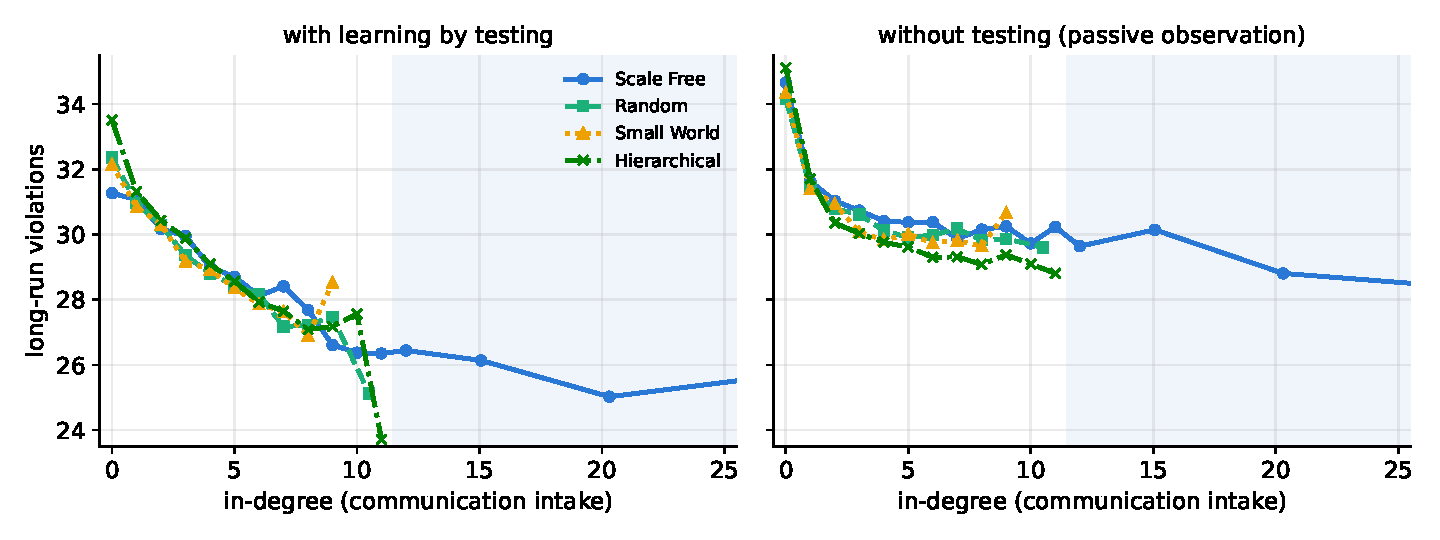
\includegraphics[width=0.9\linewidth]{figs/curve_compare.pdf}
  \caption{\textbf{The position premium requires verification.} Long-run violations versus in-degree with the full model (left) and with verification removed (right; passive observation, same recency communication), on the same networks and seeds. Without verification the curve flattens beyond the first link and the best performer's position is no longer predictable.}
  \label{fig:compare}
\end{figure}

\subsection{Analytical results}\label{sec:theory}

\todo{Section intentionally left open --- full mean-field derivation in progress (AZ, JGR).}

The simulations above pose two precise analytical targets. First, the topology-independence of the population average: in a degree-resolved mean-field description, the steady state should be a fixed point of the local update statistics from which the degree-dependent interaction rate drops out, making the long-run level identical across degree classes and hence across topologies. Second, the universal position curve: under drift, the binding state variable is the \emph{validity} of an agent's knowledge --- the fraction of its held constraints that still exist --- which rises with communication intake; a per-degree-class validity term should therefore reproduce the observed decline of violations with $k/\langle k_{\text{in}}\rangle$ and its collapse across networks (Fig.~\ref{fig:collapse}).

\begin{figure}[H]
  \centering
  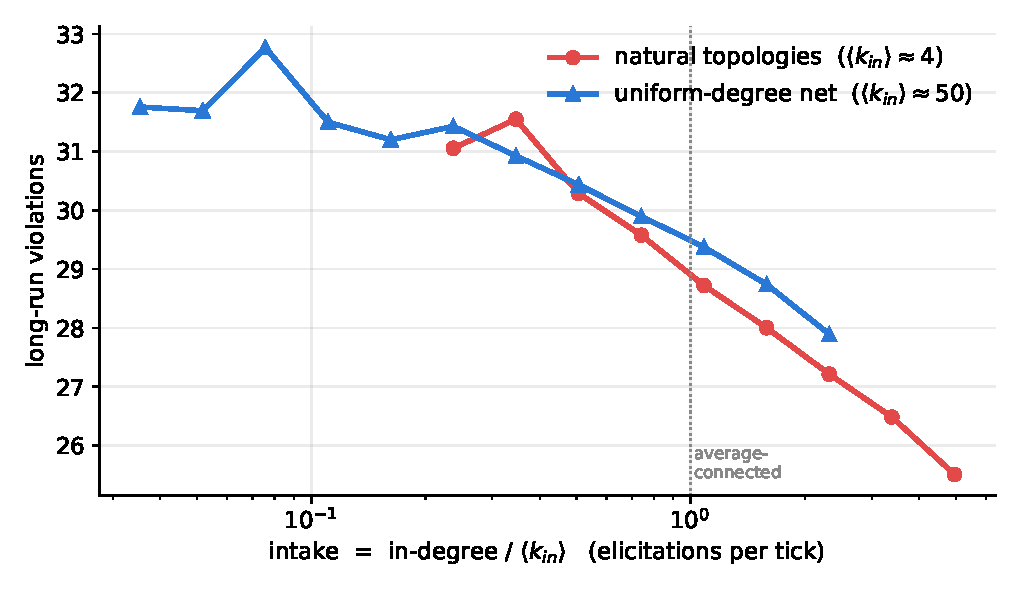
\includegraphics[width=0.62\linewidth]{figs/curve_intake_collapse.pdf}
  \caption{\textbf{The target of the theory: a single curve in intake units.} Long-run violations versus communication intake ($k/\langle k_{\text{in}}\rangle$, log scale) for networks with $\langle k_{\text{in}}\rangle \approx 4$ and $\approx 50$: the position--performance relationships collapse onto one curve. \todo{overlay analytical prediction when available}}
  \label{fig:collapse}
\end{figure}

\todo{Derivation to insert here: (i) rate equation and fixed-point argument for the mean; (ii) validity state $q_k$ and the predicted intake gradient; (iii) comparison of predicted vs.\ simulated curves.}


\section{Discussion}\label{sec:discussion}

Our central result is a dissociation. Once communication volume is equalised, the \emph{shape} of a communication network is irrelevant to how well the collective performs on average --- across canonical topologies, across a thirteen-fold range of density, and regardless of whether agents merely listen or actively verify. What the shape controls is the \emph{distribution} of performance across members: every network rewards communication intake along the same universal curve, and architecture determines which intake levels exist and who occupies them.

This reframes the classic organisational-design question. Centralisation does not buy collective performance: in our runs the scale-free networks were, if anything, marginally worse on average, because the arithmetic is conservative --- concentrating intake on hubs necessarily starves a periphery, and the gains and losses cancel along the same curve. What centralisation buys is \emph{intentionality}. In a degree-homogeneous network, being the best-informed member is an accident of small random degree differences; in a centralised one, the high-intake seats are designed objects, and whoever is placed in them will predictably outperform the periphery by a substantial margin (${\sim}5$ violations, ${\sim}15\%$, in our setting --- with the occupant of the top seat identifiable from the wiring diagram alone). When decision rights, control, or attention are scarce and must be allocated to few members, this is exactly the property a designer wants: hierarchy as an \emph{allocation instrument} rather than a performance technology. This nuances both the efficiency view of hierarchy \parencite{simon1962architecture, bolton1994firm} --- hierarchy is efficient here not because it processes information better in aggregate, but because it concentrates informational advantage where the designer intends --- and the network-performance literature's search for the ``best'' topology \parencite{lazer2007network, barkoczi2016social}: at matched communication rates there is no best topology, only different allocations of the same total.

Two scope conditions discipline the story. First, the position premium exists only among \emph{verifying} agents: when knowledge cannot be checked and disconfirmation cannot spread, extra connectivity delivers stale hearsay and the premium collapses to a connected/isolated cliff. Investments in members' capacity to test and to transmit negative results are, on this account, complements to structural centralisation --- the hub seat is only worth designing if its occupant can verify what flows through it. Second, the premium is a creature of \emph{change}: intake matters because knowledge decays, and the faster the environment drifts, the steeper the universal curve. In a static environment everyone eventually knows everything and position is worthless; in a volatile one, the allocation power of architecture is at its peak. \parencite{fang2010balancing, shore2015facts}

Our limitations point at future work. The layered generator we label ``hierarchical'' is degree-homogeneous --- it has layers but no hubs --- and correspondingly behaves like a random network throughout; a generator with genuine degree asymmetry between layers (and directed up/down flow) is needed to speak to hierarchy in the organisational sense. The communication-rate normalisation, which does the analytic work of separating volume from structure, is itself a modelling choice: in real organisations bandwidth is endogenous and may concentrate on valuable members, compounding the positional advantage we isolate here. Agents are homogeneous and non-strategic; heterogeneous testing capacity (we find, in preliminary experiments, that \emph{where} extra verification capacity sits in the network matters in non-obvious ways), endogenous link formation, and tasks with heterogeneous stakes are natural extensions. Finally, the analytical programme of Section~\ref{sec:theory} --- deriving the universal curve and its collapse from a validity-augmented mean field --- will determine how far these conclusions generalise beyond the present task family.


\section{Methods}\label{sec:methods}

\subsection{Task and environment}

All agents face the same constraint-satisfaction task over $K=30$ binary variables. The hidden constraint set $\mathcal{C}$ contains $M = \alpha K = 60$ clauses ($\alpha = 2$), each over two distinct variables joined by \textsc{and} (satisfied iff both bits are 1) or \textsc{xor} (satisfied iff the bits differ), drawn uniformly from the universe $\mathcal{U}$ of all $2\binom{K}{2} = K(K-1) = 870$ such clauses with a 50/50 operator mix. Agent $i$'s \emph{true violation count} $V_i$ is the number of clauses of $\mathcal{C}$ violated by its private assignment $x^{(i)}$. \emph{Homogeneity} is the population share of agents holding the majority value, averaged over variables. Drift: every $\tau$ ticks (default $\tau=1$) one uniformly chosen clause of $\mathcal{C}$ is replaced by a fresh draw from $\mathcal{U}$.

\subsection{Agents: signed beliefs and verification}

Agent $i$ maintains a belief store $\mathcal{B}_i \subseteq \mathcal{U}$ with signs $\sigma_i : \mathcal{B}_i \to \{+1,-1\}$; positive beliefs $\mathcal{P}_i$ (``exists'') are the agent's working constraint set, negative beliefs (``does not exist'') are epistemic records. Capacity is $|\mathcal{B}_i| \leq 2M$, evicting first-in-first-out with recency refresh (a belief returns to the back of the queue whenever it is set, confirmed, or updated). Only positive beliefs enter optimisation.

Each tick, an agent (in random activation order) performs one \emph{test} --- with probability $1/2$ a \emph{new-clause test}: draw $c$ uniformly from $\mathcal{U} \setminus \mathcal{B}_i$ and adopt $\sigma_i(c) = +1$ iff $c \in \mathcal{C}$ (probability ${\approx} M/|\mathcal{U}| \approx 0.07$; failed candidates are discarded without record); with probability $1/2$ a \emph{belief test}: draw $c$ uniformly from $\mathcal{B}_i$ and set $\sigma_i(c)$ to the ground truth, so stale positives are falsified (kept as negatives) and wrong negatives corrected. Whenever a clause becomes an active constraint (new positive or restored positive), the agent runs a local greedy repair: each variable of the clause, in random order, is flipped iff the flip strictly reduces violations over the positive beliefs sharing a variable with it.

Design rationale for the belief system (why falsified beliefs are kept and transmitted rather than deleted; why no negative records are made for never-held clauses; why capacity is doubled) follows the companion model note; briefly: deletion is invisible to the network and dead clauses are promptly re-imported from untested neighbours, negatives on never-held clauses would flood the store (non-existent clauses outnumber real ones ${\sim}13{:}1$), and the doubled cap prevents negative beliefs from mechanically crowding out positive knowledge. \todo{decide whether to cite the model note as SI or fold its full text into SI}

\subsection{Communication}

Communication is receiver-pull with rate normalisation. Each tick, for each in-neighbour $j$ of agent $i$, the link fires with probability $\min(1, s\, w_{ji})$ where all weights are $1$ and $s = 1/\langle k_{\text{in}} \rangle$ is a global scale set at construction, so the average agent absorbs one successful elicitation per tick on every network; an individual's expected intake is $k_i/\langle k_{\text{in}}\rangle$. On firing, $i$ receives $j$'s \emph{most recently acquired} belief among the \emph{disagreements} $D_{ij} = \{c \in \mathcal{B}_j : \sigma_j(c) \neq \sigma_i(c) \text{ or } c \notin \mathcal{B}_i\}$ (recency rule), and adopts $j$'s sign, running the greedy repair if this activates a constraint. Communication transmits beliefs, not ground truth: misinformation of either sign can travel and is corrected only by testing.

The predecessor (``original'') model used for comparisons replaces testing with passive observation --- with probability $p_{\text{obs}} = 0.01$ per tick the agent learns a uniformly drawn clause of $\mathcal{C}$ --- has unsigned knowledge capped at $M$ with strict FIFO, no unlearning, and (in its historical form) uniform-random rather than recency communication; both communication variants are reported where relevant. All variants are toggles of one implementation, so paired comparisons run on identical networks and seeds.

\subsection{Networks}

Natural topologies ($N=80$--$100$, matched at $\langle k_{\text{in}}\rangle \approx 4$): directed Erd\H{o}s--R\'enyi ($p=0.05$); Watts--Strogatz small-world (ring degree 4, rewiring 0.1, random edge orientation); Barab\'asi--Albert scale-free (attachment $m=4$, random orientation); layered ``hierarchical'' (3 equal layers, intra-layer connection probability 0.10, inter-layer 0.03 --- note this generator is degree-homogeneous). Designed uniform-degree networks assign node $i$ in-degree $\max(1,i)$ up to $10$, $50$, or $100$ ($N \in \{100, 101\}$), with in-neighbours drawn uniformly. Structural audits (degree statistics, clustering, modularity, seed-to-seed independence) confirmed each generator produces its intended family.

\subsection{Simulation protocol and statistics}

Runs last $T=2000$ ticks; long-run statistics are time averages over the final $W=500$ ticks (per-agent violation means over the window; population average and per-tick minimum likewise). Between $8$ and $10$ seeds per condition; topology comparisons are unpaired across networks but share seed lists; mechanism comparisons (with/without verification, with/without recency) are paired on identical networks per seed. Position analyses use Spearman rank correlations with tie-corrected average ranks; binned curves require $\geq 5$ agents per bin, pooling sparse tails; series in Fig.~\ref{fig:multinet} show $\pm 1$ s.e.m.\ bands. Because Python's per-process hash randomisation feeds the model's random draws, all reported numbers pin the hash seed and average over seeds. The model is implemented in Python (Mesa, NetworkX, NumPy); an interactive browser-based animation of information flow in the model accompanies the code.

\subsection{Analytical derivation}

\todo{To be completed --- degree-resolved mean field with validity state; will summarise the derivation here with the full treatment in Supplementary Information.}


\section*{Data availability}
All simulation outputs underlying the figures, and the scripts that regenerate them, are available in the project repository. \todo{archive a release (e.g.\ Zenodo DOI) at submission}

\section*{Code availability}
Model, analysis scripts, and the interactive animation are available at \url{https://github.com/atiyabzafar/architecturesofproblemsolving}. \todo{confirm repository visibility and add release tag}

\section*{Author contributions}
\todo{to be completed --- draft: FG conceived the model extensions, implemented the simulations and analyses, and wrote the manuscript; AZ developed the mean-field theory and co-developed the model implementation; JGR developed the mean-field theory and supervised the analytical work; PA built the interactive application; all authors discussed the results and revised the manuscript.}

\section*{Competing interests}
The authors declare no competing interests.

\section*{Acknowledgements}
The authors thank the faculty of the Complexity Global School 2025 (Santa Fe Institute and Universidad de Los Andes, Bogot\'a). \todo{carry over full acknowledgements from the earlier draft as appropriate}

\printbibliography

\appendix
\section*{Supplementary information (planned)}
\begin{itemize}
  \item Full analytical derivation and stability analysis. \todo{pending}
  \item Robustness: drift-rate sweep ($\tau \in \{1, 10\}$ reported in text; wider sweep pending), no-normalisation variant, uniform-degree networks $1$--$50$.
  \item Informative intermediate designs: deletion-only unlearning (insufficient: stale share ${\sim}43\%$) and communication stubbornness (removed: marginal effect, added complexity).
  \item The predecessor model's full results, including topology-independence under stale-dominated communication.
  \item Description of the interactive animation.
\end{itemize}

\end{document}
